%%%%%%%%%%%%%%%%%%%%%%%%%%%%%%%%%%%%%%%%%%%%%%%%%%%%%%%%%%%%
%% filename:	vortrag.tex
%% template:	Mon, 07 May 2012 13:01:14 +0200
%% author:	Hermann Lorenz
%% date:	20. Nov 2012 10:00
%%%%%%%%%%%%%%%%%%%%%%%%%%%%%%%%%%%%%%%%%%%%%%%%%%%%%%%%%%%%
\documentclass[%
	ngerman%
	]{beamer}

%\setbeameroption{show only notes} 	% note{} -- Anmerkungsfolien


%%%%%%%%%%%%%%%%%%%%%%%%%%%%%%%%%%%%%%%%%%%%%%%%%%%%%%%%%%%%
%% Lokalisierung %%%%%%%%%%%%%%%%%%%%%%%%%%%%%%%%%%%%%%%%%%%
%%%%%%%%%%%%%%%%%%%%%%%%%%%%%%%%%%%%%%%%%%%%%%%%%%%%%%%%%%%%
\usepackage[utf8]{inputenc}	% Umlaute direkt eingeben
\usepackage[T1]{fontenc}	% Wörter mit Umlaute umbrechen
\usepackage[ngerman]{babel}	% deutsche Bezeichner
\usepackage[babel,german=guillemets]{csquotes}	% \enquote{}
\usepackage{libertine}
\usepackage[scaled=0.83]{beramono}


%%%%%%%%%%%%%%%%%%%%%%%%%%%%%%%%%%%%%%%%%%%%%%%%%%%%%%%%%%%%
%% Bilder %%%%%%%%%%%%%%%%%%%%%%%%%%%%%%%%%%%%%%%%%%%%%%%%%%
%%%%%%%%%%%%%%%%%%%%%%%%%%%%%%%%%%%%%%%%%%%%%%%%%%%%%%%%%%%%
\usepackage{graphicx}	% \includegraphics{bild.pdf}
\usepackage{tikz}

%-----------------------------------------------------------
% TikZ library: arrows, positioning

\usetikzlibrary{arrows,positioning,shapes.geometric,shapes,backgrounds}
\tikzset{
    %Define standard arrow tip
    >=stealth',
    %Define style for boxes
    punkt/.style={
           rectangle,
           rounded corners,
           draw=black, very thick,
           text width=6.5em,
           minimum height=2em,
           text centered},
    % Define arrow style
    pil/.style={
           ->,
           thick,
           shorten <=2pt,
           shorten >=2pt,}
}
\usetikzlibrary{fit}

%%%%%%%%%%%%%%%%%%%%%%%%%%%%%%%%%%%%%%%%%%%%%%%%%%%%%%%%%%%%
%% pdf-links %%%%%%%%%%%%%%%%%%%%%%%%%%%%%%%%%%%%%%%%%%%%%%%
%%%%%%%%%%%%%%%%%%%%%%%%%%%%%%%%%%%%%%%%%%%%%%%%%%%%%%%%%%%%
\usepackage[ngerman]{varioref}	% \vpageref{}

%%%%%%%%%%%%%%%%%%%%%%%%%%%%%%%%%%%%%%%%%%%%%%%%%%%%%%%%%%%%
%% eigene Macros %%%%%%%%%%%%%%%%%%%%%%%%%%%%%%%%%%%%%%%%%%%
%%%%%%%%%%%%%%%%%%%%%%%%%%%%%%%%%%%%%%%%%%%%%%%%%%%%%%%%%%%%
\usepackage{xspace}

\newcommand{\zB}{z.\,B.\xspace}
\newcommand{\conclusion}{\(\to\)\xspace}

\newcommand{\todo}[1]{\textcolor{red}{TODO: #1}}
\newcommand{\prove}[1]{\textcolor{red}{TODO/PROVE(#1)}}
%\newcommand{\todo}[1]{}
%\newcommand{\prove}[1]{}

\definecolor{lgray}{gray}{.3}
\newcommand{\notall}[1]{\textcolor{lgray}{#1}}
\newcommand{\eg}[1]{\textcolor{lgray}{#1}}

\newcommand{\noteparagraph}[1]{\smallskip \textbf{#1}\,\,}


\newcommand{\myContentOverviewFrame}{%
	\begin{frame}{Agenda}%
		% show only sections, no subsections
		\tableofcontents[hideallsubsections]%
	\end{frame}%
	}

\newcommand{\myContentDiscussionFrame}{%
	\begin{frame}{Diskussion und Vorführung}%
		% show only sections, no subsections
		\tableofcontents[hideallsubsections]%
	\end{frame}%
	}

\usepackage{ifthen}
% use: \myContentSectionFrame
% use: \myContentSectionFrame[1-2]
\newcommand{\myContentSectionFrame}[1][\empty]{%
	\begin{frame}{\insertsection{} -- Übersicht}%
		\ifthenelse{\equal{#1}{\empty}}%
			% show only sections, no subsections
			{\tableofcontents[currentsection,currentsubsection,hideothersubsections]}%
			% show only the given sections, but show only subsections for currentsection
			{\tableofcontents[sections={<#1>},currentsection,currentsubsection,hideothersubsections]}%
	\end{frame}%
	}

\setbeamertemplate{frametitle}{
	\hspace{-1.5em}
	\insertframetitle\\
	\hspace{-.5em}\scriptsize\insertframesubtitle\hfill\insertpart\\[-.9em]
	\rule{\textwidth}{.1pt}
}
\setbeamertemplate{frametitle}{%
	\renewcommand{\arraystretch}{0.5}
	\begin{tabular}{@{}l}
		\hspace{-1.5em}
		\insertframetitle \tabularnewline
		\hspace{-.5em}
		\scriptsize\insertframesubtitle \tabularnewline
	\end{tabular}
	\hfill%
	{\scriptsize\insertpart}\\[-.5em]
	\rule{\textwidth}{.1pt}
}
\setbeamertemplate{footline}{
	\usebeamercolor[fg]{structure}
	\hspace*{.5cm}\raisebox{3pt}{
	\begin{tikzpicture}
		\draw [draw opacity=0.0] (-2pt,0) -- (.85\textwidth + 2pt,0) -- (.85\textwidth + 2pt,-5pt) -- (-2pt,-5pt) -- cycle;
		\draw (0,0) -- (.85\textwidth,0);
		\ifnum\inserttotalframenumber>1
		\if \insertpartstartpage \insertpartendpage
		\else
		\draw [fill,xshift=.85\textwidth / (\insertpartendpage - \insertpartstartpage) * (\insertpagenumber - \insertpartstartpage)] (0,0) -- (2pt,-5pt) -- (-2pt,-5pt) -- cycle;
		\fi
		\fi
	\end{tikzpicture}
	}
	\hfill\raisebox{3pt}{\insertframenumber/\inserttotalframenumber\hspace{3pt}}
}

\definecolor{hllgreen}{rgb}{.2,.7,.2}
\definecolor{hllgreenbg}{rgb}{.9,1,.9}
\definecolor{hllblue}{rgb}{.2,.2,.7}
\definecolor{hllbluebg}{rgb}{.9,.9,1}
\definecolor{hllorange}{rgb}{1,0.482,0}
\definecolor{hllorangebg}{rgb}{1,0.782,.4}
\setbeamertemplate{blocks}[rounded]
\setbeamercolor{structure}{fg=hllblue}
\setbeamercolor{normal text}{fg=black}
\setbeamercolor{alerted text}{fg=hllorange}
\setbeamercolor{block title alerted}{fg=black,bg=hllorange}
\setbeamercolor{block body alerted}{fg=black,bg=hllorangebg}
\setbeamercolor{block title}{fg=white,bg=hllblue}
\setbeamercolor{block body example}{fg=black,bg=hllgreenbg}
\setbeamercolor{block title example}{fg=white,bg=hllgreen}
\setbeamercolor{block body}{fg=black,bg=hllbluebg}

\newcommand{\prosymbol}{%
	\raisebox{-.1\baselineskip}{%
		\begin{tikzpicture}%
			\draw [line width=.1\baselineskip] (-.25\baselineskip,0) -- (.25\baselineskip,0);%
			\draw [line width=.1\baselineskip] (0,-.25\baselineskip) -- (0,.25\baselineskip);%
		\end{tikzpicture}%
	}%
	}
\newcommand{\contrasymbol}{%
	\raisebox{.15\baselineskip}{%
		\begin{tikzpicture}%
			\draw [line width=.1\baselineskip] (-.25\baselineskip,0) -- (.25\baselineskip,0);%
		\end{tikzpicture}%
	}%
	}
\definecolor{procolor}{rgb}{0,.8,0}
\definecolor{contracolor}{rgb}{.8,0,0}
%         |
%         |
%         |
%   ------+------
%         |
%         |
%         |
%
% h = .5\baselineskip
%
%
%   -------------
% h = .1\baselineskip
%
%
\newenvironment{proconlist}%
	{%
		\begin{list}{?}{}%
		\newcommand{\pro}{\item[\textcolor{procolor}{\prosymbol}]}%
		\newcommand{\contra}{\item[\textcolor{contracolor}{\contrasymbol}]}%
	}{%
		\end{list}%
	}


\usepackage{listings}
\lstset{basicstyle=\ttfamily\scriptsize,backgroundcolor=\color[rgb]{.9,.9,.9}}
\usepackage{dirtree}

\usepackage{tabularx}
\usepackage{dcolumn}
\usepackage{multirow}
\usepackage{booktabs}
\usepackage{bbding}
\usepackage[squaren]{SIunits}

\newcommand{\theadhll}[1]{\emph{\scriptsize #1}}

%-------------------------------------------------------------------------------
% Inhaltsverzeichnis bei jeder Section
% (funktioniert leider nicht in allen Latex-Versionen einwandfrei)
%\AtBeginSection{%
%	\begin{frame}{Übersicht}%
%		\tableofcontents[currentsection]%
%	\end{frame}%
%}

%-------------------------------------------------------------------------------
% Navigationsleiste ausblenden
\setbeamertemplate{navigation symbols}{}

%-------------------------------------------------------------------------------
% Diesen Abschnitt über \begin{document} lassen, damit die PDF-Informationen
% korrekt gesetzt werden.
\title{%
	Überprüfung der Realisierbarkeit einer offenen
	Hausautomatisierungslösung durch Anwendung bestehender
	Informationstechnologien in einem Sensornetz
	}
\date{31.\,Januar~2012}
\author{Angelos~Drossos \and Hermann~Lorenz
	\and Ulrich~Meckel \and Martin~Doenicke
	\and Thomas~Bettermann \and Robert~Krampe \newline
	\and Marcus~Kupke \and Markus~Fischer
	\and Enrico~Uhlig}
\institute{Hochschule für Technik und Wirtschaft Dresden\\%
			Master Angewandte Informationstechnologien\\%
			Forschungsprojekt Sensornetze\\%
			Prof. Dr. J. Vogt%
}
%-------------------------------------------------------------------------------

\begin{document}
%-------------------------------------------------------------------------------
\begin{frame}[plain]
	\maketitle
\end{frame}

%-------------------------------------------------------------------------------
\myContentOverviewFrame
\section{Einführung}
\myContentSectionFrame

%----------------------------------------------------------

\subsection{Gebäude- vs. Hausautomatisierung}

%----------------------------------------------------------

\begin{frame}{Abgrenzung von Haus- und Gebäudeautomatisierung}{Gebäudeautomatisierung}
	\begin{itemize}
	\item 	wichtiger Bestandteil des technischen Facility-Managements
	\item 	Energie- und Personaleinsparungen stehen im Vordergrund
	\item 	dezentrale Anordnung der Steuerungseinheiten
	\item 	Funktionsabläufe gewerkeübergreifend automatisch durchführen
	\item 	Visualisierung der Automation nebensächlich\newline
			(nur in der Managementebene)
	\item 	i.\,d.\,R. herstellerspezifische, kommerzielle Bussysteme
	\item 	Trend zur Offenheit und zum herstellerübergreifenden Informationsaustausch
			(\emph{Interoperabilität}\,)
			% Lockerung der Herstellerabhängigkeit (kein OpenSource-Gedanke!)
			% Bussystem gibt die Möglichkeit, Fabrikate mehrerer Hersteller
			% ohne größere Probleme miteinander kommunizieren zu lassen.
			% Hersteller generieren für ihre Gateways je nach Projekt
			% politische Preise, um der Interoperabilität entgegen zu wirken.
	\end{itemize}
\end{frame}

%----------------------------------------------------------

\begin{frame}{Abgrenzung von Haus- und Gebäudeautomatisierung}{Hausautomatisierung}
	\begin{itemize}
	\item 	Teilbereich der Gebäudeautomatisierung
	\item 	auf spezielle Bedürfnisse der Bewohner von (privaten) Wohnhäusern zugeschnitten
	\item 	erhöhte Wohnkomfort, Sicherheit der Bewohner und Überwachung im Vordergrund
	\item 	Visualisierung und Interaktion der Bewohner besonders wichtig
	\item 	System muss skalierbar sein
	\item 	neue Geräte müssen leicht installiert werden können
	\end{itemize}
\end{frame}

%----------------------------------------------------------

\subsection{Motivation und Ziel}

\begin{frame}{\insertsubsection}{Vorüberlegungen zur Hausautomatisierung}
	\begin{exampleblock}<+->{bestehende Hausautomatisierungslösungen}
	bestehende Heimautomatisierungen besitzen mindestens einen, meist
	mehrere der folgenden, gravierenden Nachteile:
	\begin{itemize}
	\item	teuer
	\item	proprietär
	\item	schlecht dokumentiert
	\item	wenig Sicherheit (\zB in der Datenübertragung)
	\end{itemize}
	\end{exampleblock}

	% neue Netzwerktechnologien (CoAP, 6LoWPAN, \dots) legen die Möglichkeit
	% nahe, mit ihrer Hilfe eine offene Lösung zu konzipieren

	\begin{block}<+->{Wunsch nach \enquote{freier} Hausautomatisierung}
		\begin{itemize}
		\item 	Hersteller-Unabhängigkeit (Interoperabilität)
		\item 	geringere Installationskosten
		\item 	überschaubarer Wartungsaufwand
		\item 	Regelverarbeitung soll möglichst leicht konfigurierbar sein
		\item 	Stichwort \emph{Internet der Dinge}
		\end{itemize}
	\end{block}
\end{frame}


\section[Ansatz]{Ansatz}
\myContentSectionFrame[\thesection - 6]

%----------------------------------------------------------
%----------------------------------------------------------

\subsection[Anforderungen]{Anforderungen an das Hausautomatisierungssystem}

%----------------------------------------------------------

\begin{frame}{\insertsection}{Anforderungen I}
	\begin{block}<+->{Dedizierter Netzknoten zur Regelung und Kontrolle}
		\begin{itemize}
		\item 	für den Hausbewohner leicht konfigurierbar und wartbar
		\item 	Netzknoten befindet sich außerhalb des Sensornetzes
		\end{itemize}
	\end{block}
	\vfill
	\begin{block}<+->{Integration bestehender Sensornetze}
		\begin{itemize}
		\item 	Gewährleistung der Interoperabilität
		\item 	Verringerung der Anschaffungskosten bei vorhandenen Sensornetzen
		\end{itemize}
	\end{block}
\end{frame}

%----------------------------------------------------------

\begin{frame}{\insertsection}{Anforderungen II}
	\begin{block}<+->{Verwendung \enquote{klassischer} Internetprotokolle}
		\begin{itemize}
		\item 	Verwendung auf Vermittlungs-, Transport- und Anwendungsschicht
		\item 	Erhöhung der Transparanz und Annahmebereitschaft der Hausbewohner
		\item 	Einsparung von zusätzlichem Entwicklungsaufwand
				% man betrachte heutzutage die vielen unterschiedlichen Betriebssyteme
				% Mac OS, Windows, Linux Derivate, Android, iOS, BlackBerry, Firefox OS, Chrome OS
		\item 	Analyse klassischer Internetprotokolle\newline
				für den Einsatz in Sensornetzen
				% Batterielebensdauer / Radio Duty Cycle / etc.
		\end{itemize}
	\end{block}
	\vfill
	\begin{block}<+->{Ausfall und Erweiterbarkeit von Netzknoten im Sensornetz}
		\begin{itemize}
		\item 	Wunsch nach Sicherheit (verschlüsselte Übertragung und Authentifizierung)
		\item 	Einfache Installation neuer Sensor-/Aktorknoten
		\item 	Flexibles Routing im Sensornetz
		\end{itemize}
	\end{block}
\end{frame}

%----------------------------------------------------------

\subsection{Verwandte Arbeiten}

%----------------------------------------------------------

	\subsubsection{FHEM}

%----------------------------------------------------------

\begin{frame}{\insertsubsection}{\insertsubsubsection}
	\uncover<1->{\enquote{FHEM ist ein Hausautomations-Server,
		geschrieben von Rudolf Koenig et al. in Perl,
		um FS20-Komponenten und andere Geräte zu steuern.}}
	\uncover<2->{\begin{proconlist}
	\pro 	Dedizierter Netzknoten zur Regelung und Kontrolle
	\pro 	Integration bestehender Sensornetze (FS20, HomeMatic)
	\contra Ausfall und Erweiterbarkeit von Netzknoten:
			\begin{itemize}
			\item 	Regelverarbeitung durch Skriptsprache
			\item 	Komplexe Regeln müssen in Perl implementiert werden
			\end{itemize}
	\contra Verwendung \enquote{klassischer} Internetprotokolle:
			\begin{itemize}
			\item 	es müssen Gateways bereitgestellt werden,
					die beide Netzwerkstacks implementieren
			\item 	keine Transparenz vorhanden
			\item 	Gateways wirken der Interoperabilität entgegen
			\end{itemize}
	\end{proconlist}
	\begin{itemize}
	\item 	Projekt-Seite: \url{http://www.fhemwiki.de/wiki/FHEM}
	\item 	Lizenz: GPLv2
	\end{itemize}}
\end{frame}

%----------------------------------------------------------

	\subsubsection[Hexabus]{Hexabus -- the Kranken of Automation}

%----------------------------------------------------------

\begin{frame}{\insertsubsection}{\insertsubsubsection}
	\uncover<1->{\enquote{An IPv6-based home automation bus.}}
	\uncover<2->{\begin{proconlist}
	\contra 	befindet sich noch im Aufbau
	\contra Kein dedizierter Netzknoten zur Regelung und Kontrolle
			\begin{itemize}
			\item 	Regelverarbeitung verteilt auf verschiedene Knoten
			\item 	erfordert eine Übersicht über alle Knoten beim Anwender
			\end{itemize}
	\contra Keine Integration bestehender Sensornetze
	\pro 	Ausfall und Erweiterbarkeit von Netzknoten durch Routing-Protokoll gelöst
	\pro 	Es werden \enquote{klassische} Internetprotokolle verwendet:
			\begin{itemize}
			\item 	es wird die IPv6-Technologie angewandt: 6LoWPAN
			\item 	Transparenz auf Vermittlungs- und Transportschicht
			\item 	Anwendungsschicht (Hexabus Protokoll): nicht klassisch
			\end{itemize}
	\end{proconlist}
	
	\begin{itemize}
	\item 	Projekt-Seite: \url{https://github.com/mysmartgrid/hexabus/wiki}
	\end{itemize}}
\end{frame}

%----------------------------------------------------------

\subsection{Projekteinteilung}

%----------------------------------------------------------

\begin{frame}{\insertsection}{\insertsubsection}
	\begin{block}{dedizierter Regelungsserver}
		\begin{enumerate}
		\item 	DB zur Verwaltung der Sensoren/Aktoren
		\item 	Integrierung der Anwendungsschicht (CoAP)
		\item 	Regelverarbeitung (inkl. Weboberfläche)
		\end{enumerate}
	\end{block}
	\begin{block}{Gateway zur Integration bestehender Sensornetze}
		\begin{enumerate}
		\item 	FS20
		\item 	HomeMatic
		\end{enumerate}
	\end{block}
	\begin{block}{Eigenes drahtloses Sensornetz (WSN)}
			\begin{enumerate}
			\item 	Border Router
			\item 	Routerknoten
			\item 	Netzknoten mit Sensoren
			\item 	Netzknoten mit Aktoren
			\end{enumerate}
	\end{block}
\end{frame}

%----------------------------------------------------------

%\subsection{Aufgabenstellung}

%----------------------------------------------------------

%\begin{frame}{\insertsubsection}{}
%	\begin{itemize}
%	\item	prüfen, ob mit bestehenden, offenen Technologien der Aufbau
%		einer Heimautomatisierung möglich erscheint
%	\item	als Sensoren und Aktoren sollen Funkmodule genutzt werden
%	\item	Datensicherheit im Konzept von vornherein vorsehen
%	\item	Praxisnähe
%		\begin{itemize}
%		\item	bestehende Technologien kombinieren um Aufwand zu sparen
%		\item	offene Standards verwenden, um anderen die Mitarbeit
%			kostengünstig zu ermöglichen
%		\item	auf Energiesparsamkeit achten, da Knoten mit Batterien
%			laufen
%		\end{itemize}
%	\end{itemize}
%\end{frame}

%-------------------------------------------------------------------------------

% Ausblick
% - Entwicklung eines "neuen" MAC-Protokolls in Contiki, welches dem 6LoWPAN-Standard entspricht
%   und auch energie-effizient arbeitet und einer bestimmten MAC-Protokollgruppe angehört.


\section{Hausautomatisierungslösung}
\myContentSectionFrame[\thesection - 6]

%----------------------------------------------------------

\subsection{Systemarchitekur}{Dedizierter Steuerungsserver}

%----------------------------------------------------------

\begin{frame}[label=netzwerkaufbau]{\insertsubsection}{}
\begin{tikzpicture}[funk/.style={dashed},
	knoten/.style={draw,rectangle,font=\scriptsize},
	pc/.style={draw,rectangle},
	gateway/.style={draw,ellipse,font=\scriptsize},
	protokoll/.style={pos=.5,above,sloped,font=\tiny},
	node distance=2cm]
	%,every node/.style={scale=.5}]

%-------------------------------------------------------------------------------
% IPv6 - Network
%-------------------------------------------------------------------------------
\coordinate (ipv6anfang)	at (0,0);
\coordinate (ipv6mitte)		at (2,0);
\coordinate (ipv6ende)		at (4,0);
\draw [very thick] (ipv6anfang) -- node [protokoll,below] {IPv6} (ipv6mitte) -- (ipv6ende);

\node (internet) [draw, cloud, aspect=2, below of=ipv6mitte,yshift=.5cm,xshift=.5cm]	{Internet};
\draw (internet) -- (2.5,0);
\node (server) [pc,above of=ipv6mitte,yshift=-.8cm]			{Server};
\draw (server) -- (ipv6mitte);

%-------------------------------------------------------------------------------
% 6LoWPAN - Network
%-------------------------------------------------------------------------------
\node (6lpproxy) [gateway,	above of=ipv6ende,yshift=-.8cm]		{Proxy};
\draw (6lpproxy) -- (ipv6ende);

\node (6lpbr) [knoten, above of=6lpproxy,yshift=-.5cm]	{BR};
\draw (6lpbr) -- node [protokoll] {USB} (6lpproxy);

\node (6lpr) [knoten, above right of=6lpbr] {R};
\draw [funk] (6lpr) -- node [protokoll] {6LoWPAN} (6lpbr);

\node (6lpl1) [knoten, right of=6lpr] {L};
\draw [funk] (6lpl1) -- node [protokoll] {6LoWPAN} (6lpr);
\node (6lpl2) [knoten, below right of=6lpbr] {L};
\draw [funk] (6lpl2) -- node [protokoll] {6LoWPAN} (6lpbr);

\begin{pgfonlayer}{background}
	\node[fill=green!20,rounded corners] (background) [fit=(6lpproxy) (6lpbr) (6lpr) (6lpl1) (6lpl2)] {};
	\node [rotate=-90,anchor=south] at (background.east) {6LoWPAN};
\end{pgfonlayer}

%-------------------------------------------------------------------------------
% FS20 - Network
%-------------------------------------------------------------------------------
\node (fs20gw) [gateway,	above of=ipv6anfang,yshift=-.8cm]		{GW};
\draw (fs20gw) -- (ipv6anfang);

\node (fs20br) [knoten, left of=fs20gw, xshift=.3cm]	{BR};
\draw (fs20br) -- node [protokoll] {USB} (fs20gw);

\node (fs20l1) [knoten, above of=fs20br] {L};
\draw [funk] (fs20l1) -- node [protokoll] {FS20} (fs20br);
\node (fs20l2) [knoten, above right of=fs20br] {L};
\draw [funk] (fs20l2) -- node [protokoll] {FS20} (fs20br);

\begin{pgfonlayer}{background}
	\node[fill=red!20,rounded corners] (background) [fit=(fs20gw) (fs20br) (fs20l1) (fs20l2)] {};
	\node [rotate=90,anchor=south] at (background.west) {FS20};
\end{pgfonlayer}

%-------------------------------------------------------------------------------
% HomeMatic - Network
%-------------------------------------------------------------------------------
\node (hmgw) [gateway,	below of=ipv6anfang]		{GW};
\draw (hmgw) -- (ipv6anfang);

\node (hmbr) [knoten, left of=hmgw, xshift=.3cm]	{BR};
\draw (hmbr) -- node [protokoll] {USB} (hmgw);

\node (hml) [knoten, above of=hmbr,yshift=-.8cm] {L};
\draw [funk] (hml) -- node [protokoll] {HM} (hmbr);

\begin{pgfonlayer}{background}
	\node[fill=blue!20,rounded corners] (background) [fit=(hmgw) (hmbr) (hml)] {};
	\node [rotate=90,anchor=south] at (background.west) {HomeMatic};
\end{pgfonlayer}
\end{tikzpicture}

\end{frame}

%----------------------------------------------------------

\subsection[REST]{REST Programmierparadigma im Sensornetz}


\begin{frame}{\insertsubsection}{}
% Warum ist das REST Programmierparadigma sinnvoll im Sensornetz
		\begin{block}<+->{Adressierbarkeit}
			\begin{itemize}
        		\item jeder REST-Dienst eines Servers hat eindeutige Adresse (URI)
        		\item Sensoren und Aktoren haben feste Adresse % unter der sie erreichbar sind
    			\end{itemize}
		\end{block}
		\begin{block}<+->{Zustandslosigkeit}
    			\begin{itemize}
        		\item zustandslose Anfragen
        		\item jeder Request ist in sich geschlossen
        		\item Request enthält alle Informationen für die Verarbeitung
    			\end{itemize}
		\end{block}
		\begin{block}<+->{Operationen}
    			\begin{itemize}
        		\item REST-Server beschreiben ihre Dienste auf Anfrage
        		\item standardisierte Anfragemöglichkeiten\newline
				(GET / PUT / POST / DELETE)
        		\item Sensoren/Aktoren können mit GET abgefragt werden
        		\item Aktoren können mit PUT geschaltet werden
    			\end{itemize}
		\end{block}
\end{frame}



% CoAP : http://datatracker.ietf.org/doc/draft-ietf-core-coap/
\begin{frame}{Constrained Application Protocol (CoAP)}{}
        \begin{proconlist}
            \pro REST Paradigma, aber \enquote{leichtgewichtiger} als HTTP
            \pro einfaches HTTP-Mapping möglich, laut RFC-draft vorgesehen
            \pro optionale Zuverlässigkeitsmechanismen (Confirmable / Non-Confirmable)
            \pro Interoperabilität
            \pro entspricht dem Ansatz \emph{Internet der Dinge}
            \pro geringer Overhead gegenüber
HTTP\footnote{\url{http://www.comnets.uni-bremen.de/itg/itgfg521/aktuelles/fg-workshop-29092011/ITG_HH_thomas_poetsch.pdf}}
            \procon noch in Entwicklung (wird ständig verbessert, jedoch ggf. veraltete Implementierungen)
            \contra größerer Overhead als Eigenentwicklung\newline
			(jedoch mangelnde Interoperabilität)
        \end{proconlist}
\end{frame}



%----------------------------------------------------------

\subsection[Regelwerk]{Regelverarbeitungssystem}

%----------------------------------------------------------
\begin{frame}{\insertsubsection}{Ziel}
	\begin{itemize}
	\item	automatische Ansteuerung von Knoten über vorher festgelegte
		Regeln
		\begin{itemize}
		\item	Festlegung von Bedingungen
		\item	Ausführen einer (oder mehrerer) Aktionen bei Erfüllung
		\item	(evtl. alternative Aktionen bei Nichterfüllung)
		\end{itemize}
	\item	flexible Anpassung dieser Regeln
		\begin{itemize}
		\item	manuell für erfahrene Benutzer
		\item	über einfach zu bedienende (Web-)Oberfläche für
			Endanwender
		\end{itemize}
	\end{itemize}
\end{frame}
%----------------------------------------------------------
\begin{frame}{\insertsubsection}{Aufbau}
	\begin{itemize}
	\item	Beschreibung von Regeln in XML-Datei
	\item	Syntax in DTD definiert
	\item	flexible und eindeutige Kommunikation
	\end{itemize}
	\lstinputlisting[language=xml,tabsize=4]{bsp/regeln.dtd}
\end{frame}
%----------------------------------------------------------
\begin{frame}{\insertsubsection}{Kommunikation}
	\definecolor{gruen}{rgb}{0,.8,0}
\definecolor{orangig}{rgb}{1,.452,0}
\begin{tikzpicture}[>=stealth',pc/.style={rectangle,minimum width=1.5cm, minimum height=5cm,draw},%
	mynode/.style={rectangle,draw, minimum width=1.5cm},
	nachricht/.style={font=\scriptsize,auto}
	]
	\node (client) [pc]		{Client};
	\node (webserver) [pc]		[right of=client, xshift=2.5cm] {\parbox{\widthof{Server}}{Web-Server}};
	\node (pythonserver) [pc]	[right of=webserver, xshift=2.5cm] {\parbox{\widthof{Python-}}{Python-Server}};
	\node (db) [rectangle,draw, minimum height=.8cm, minimum width=2.5cm, below of=webserver,xshift=1.8cm,yshift=-3cm] {Datenbank};

	\node (node1) [mynode,right of=pythonserver,xshift=2cm,yshift=2.25cm]	{Node};
	\node (node2) [mynode,below of=node1]		{Node};
	\node (node3) [mynode,below of=node2]		{Node};

	\draw [<->,shorten >=1mm,shorten <=1mm] (client.north east) -- node [auto] {HTTP} (webserver.north west);
	\draw [<->,shorten >=1mm,shorten <=1mm] (webserver.north east) -- node [auto] {Web-Socket} (pythonserver.north west);
	\draw [<->,shorten >=1mm,shorten <=1mm] (pythonserver.north east) -- node [auto] {6LoWPAN} (node1.north west);

	\draw [<->,shorten >=1mm,shorten <=1mm] (db.north west) -- node [sloped,above,font=\tiny] {SQLite} (webserver);
	\draw [<->,shorten >=1mm,shorten <=1mm] (db.north east) -- node [sloped,above,font=\tiny] {SQLite} (pythonserver);

	\uncover<2->{
		\draw [->,orangig] (client) -- node [nachricht] {Web-Request} (webserver);
		\draw [->,orangig] (webserver) -- node [nachricht] {\parbox{\widthof{Nachricht}}{\centering Socket-Nachricht}} (pythonserver);
		\draw [orangig] (pythonserver.east){}+(0.1,0.1) edge [bend left, ->, shorten >=1mm] node [above, font=\scriptsize] {\parbox{1.5cm}{\centering CoAP-Anfrage}} (node3.west);
	}

	\uncover<3->{
		\draw [gruen] (pythonserver.south east){}+(0,-0.1) edge [bend left,->,shorten >=1mm] node [auto,font=\scriptsize] {Eintrag in DB} (db.east);
		\draw [gruen] (db.west){}+(-0.1,0) edge [bend left,->,shorten >=1mm] node [below,font=\scriptsize,xshift=-.2cm,yshift=-.3cm] {\parbox{2cm}{\centering Auslesen der Sensorwerte aus DB}} (webserver.south west);
		\draw [gruen] (client.south east){}+(0.1,0.1) edge [bend left,->,shorten >=1mm,font=\scriptsize] node [above] {\parbox{1.6cm}{\centering Zyklisches Nachladen der Seite}} (webserver.south west);
		\draw [gruen] (webserver.south west){}+(-0.1,-0.1) edge [bend left,->,shorten >=1mm] (client.south east);
		\draw [gruen] (node3.west){}+(-0.1,-0.1) edge [bend left, ->, shorten >=1mm] node [below, font=\scriptsize] {\parbox{1.5cm}{\centering CoAP-Antwort}} (pythonserver.east);
	}
\end{tikzpicture}

\end{frame}
%----------------------------------------------------------
\begin{frame}{\insertsubsection}{Umsetzung}
	\begin{columns}
	\column{.45\textwidth}
		\begin{block}{zentral}
		\begin{proconlist}
		\pro	Verwaltung an zentraler Stelle
		\pro	einfache Client-Anwendungen
		\pro	weniger Kommunikation im Netz
		\end{proconlist}
		\end{block}
	\column{.45\textwidth}
		\begin{block}{dezentral}
		\begin{proconlist}
		\pro	Ausfall eines Steuerungsknotens tolerierbar
		\pro	Autonome Systeme möglich
		\contra	benötigt Broadcast-Kommunikation
		\end{proconlist}
		\end{block}
	\end{columns}
\end{frame}
%----------------------------------------------------------

\section{Bestehende Sensornetze} % wie FS 20 und HM
\myContentSectionFrame[\thesection - 6]

\againframe{netzwerkaufbau}
%-------------------------------------------------------------------------------

\begin{frame}{\insertsubsection}{Interessante Fragestellungen}
	\begin{itemize}
	\item 	Ist es möglich, bestehende Sensornetztechnologien in unseren Ansatz zu integrieren?
	\item 	Welche Vor- und Nachteile bietet die Integration solcher Technologien?
	\item 	Was bringt der Einsatz von CoAP zum Ansprechen der Fremdkomponenten?
	\end{itemize}
	\vspace{0.5em}
	\begin{center}
		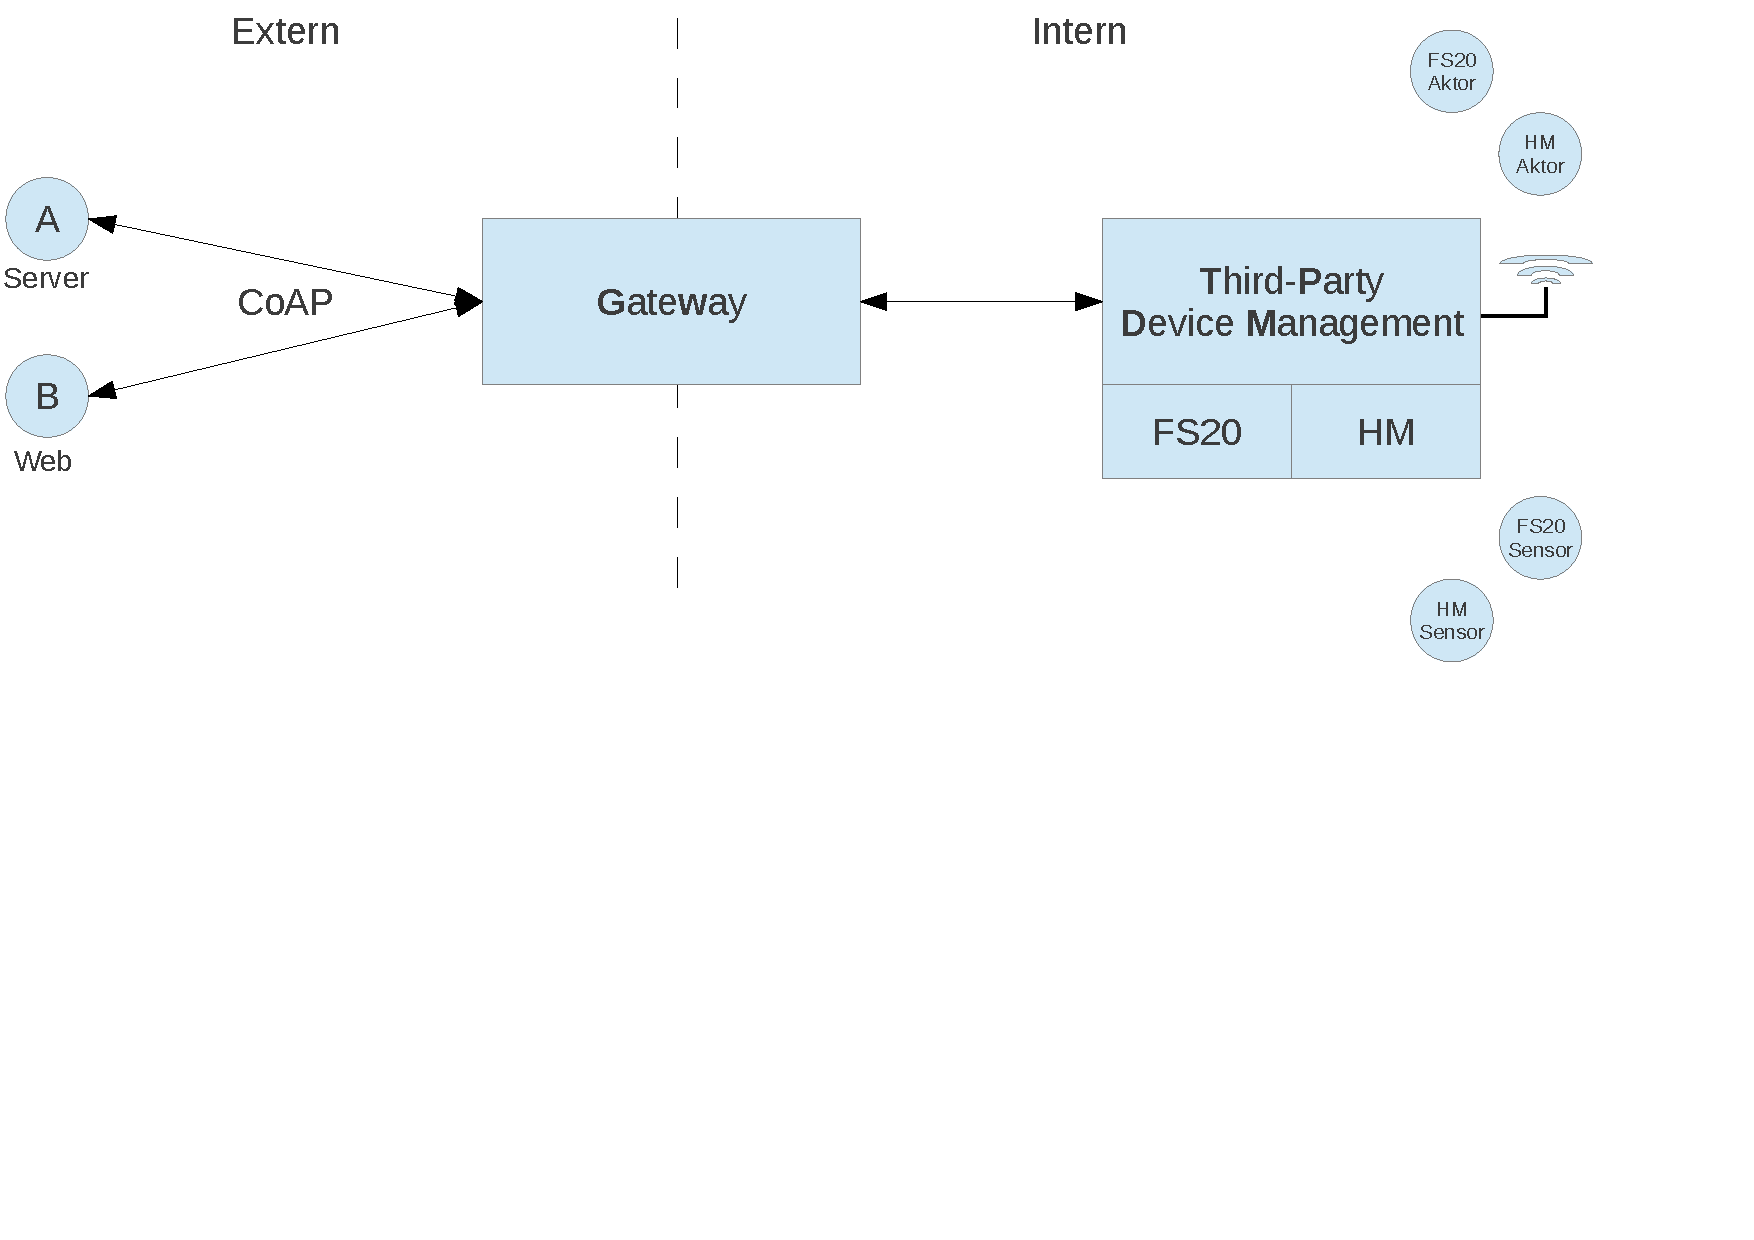
\includegraphics[scale=0.38]{pic/gateway_ueberblick}
	\end{center}
\end{frame}

%-------------------------------------------------------------------------------

\begin{frame}{Gateway in bestehenden Sensornetzen}{Lösungsansätze HomeMatic/FS20}
	\begin{itemize}
	\item 	Reverse-Engineering
		\begin{itemize}
		\item 	Mitlesen von Nachrichten
		\item 	Analyse des HomeMatic-Protokolls
		\item 	Heranziehen alternativer Informationsquellen
		\end{itemize}
	\item Erkenntnisse in Programm umsetzen
		unter Berücksichtigung der Anbindung zum Gateway
\end{itemize}
\end{frame}


%-------------------------------------------------------------------------------

\begin{frame}{\insertsubsection}{Ergebnisse I}
	\begin{itemize}
	\item 	Integration von bestehenden Sensornetztechnologien ist möglich, aber aufwendig
	\end{itemize}
	\vspace{1em}
	Nutzung von bestehenden Sensornetzen:
	\begin{proconlist}
	\pro 	Reduzierung Entwicklungsaufwand der Hardware
	\pro 	Vorteile des jeweiligen Systems nutzbar
	\pro 	Systemübergreifender Einsatz
	\contra Verzicht auf Funktionalität
	\contra hoher Aufwand bei geschlossenen Systemen
	\end{proconlist}
\end{frame}

%-------------------------------------------------------------------------------

\begin{frame}{\insertsubsection}{Ergebnisse II}
	\begin{itemize}
	\item 	Gateway (CoAP $ \leftrightarrow $ bestehende Sensornetze)
	\end{itemize}
	\vspace{1em}
	\begin{proconlist}
	\pro 	standardisierte Schnittstelle für den Zugriff auf die Fremdkomponenten
	\contra für jedes System und Geräteklasse ist Ressource (PUT/GET) zu implementieren
	\end{proconlist}
\end{frame}

\section{6LoWPAN}

\subsection{Routing (RPL)}

\begin{frame}{Routing in 6LoWPAN}{RPL}
		\begin{block}{}
			\begin{itemize}
			\item 	dynamisches Routing-Protokoll
					für energiearme und verlustbehaftete Netzwerke
			\item 	Route-Over-Protokoll
			\item 	Protokoll auf Basis eines Distanzvektor-Algorithmus:
					\begin{itemize}
					\item 	DODAG (Destination Oriented Directed Acyclic Graph)
					\item 	jeder Knoten besitzt einen Rang
					\item 	spezielle Nachrichten zum Austausch der
							Routing-Informationen \eg{(DIO, DIS, DAO)}
					\item 	Zielfunktion berechnet Rang
							und wählt bevorzugten Elternknoten
					\end{itemize}
			\item 	weitere Besonderheiten:
					\begin{itemize}
					\item 	Local und Global-Repair (z.B. bei Ausfall eines Knotens)
					\item 	Verwendung des Trickle Timer Algorithmus
					\end{itemize}
			\item 	Implementation in Contiki: ContikiRPL
					\begin{itemize}
					\item 	keine im Standard definierten Sicherheitsmechanismen implementiert
					\end{itemize}
			\end{itemize}
		\end{block}
\end{frame}

\begin{frame}{Routing in 6LoWPAN}{RPL}
	\begin{figure}
	\centering
	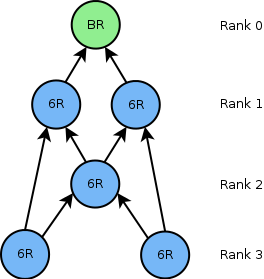
\includegraphics[width=0.5\linewidth]{Dodag}
	\linebreak
	\emph{Ein Beispielnetz}
	\end{figure}
\end{frame}
\subsection{Sensorknoten}

\begin{frame}{Sensorknoten letztes Semester}
	\begin{itemize}
	\item 	Sensor Terminal Board
			mit rcb128rfa1 Modul
	\item 	AVR ATmega128rfa1 Microcontroller
	\item 	Ansteuerung der Sensoren
			ohne Betriebssystem:
			\begin{itemize}
			\item 	Feuchtigkeitssensor
			\item 	Drucksensor
			\item 	Geschwindigkeitssensor
			\item 	Ansteuerung per I2C-Bus
			\end{itemize}
	\item 	Einarbeitung in Contiki:
			\begin{itemize}
			\item 	Wie können die Sensoren sinnvoll implementiert werden?
			\item 	Beachtung der Trennung von
					Core, CPU und Platform
			\item 	Nutzung bereits implementierter Schnittstellen
			\end{itemize}
	\end{itemize}
\end{frame}

\begin{frame}{Sensorknoten dieses Semester}
	\begin{itemize}
	\item 	deRFmega128-Board (Batteriebetrieb)
	\item 	AVR ATmega128rfa1 Microcontroller
	\item 	Verifizierung der I2C-Schnittstelle in Contiki durch neuen Sensor (Lichtsensor)
	\item 	Ansteuerung eines Aktors (Heizungsthermostat):
			\begin{itemize}
			\item 	zwei Boards, die per UART miteinander kommunizieren
			\item 	Software des Heizungsthermostat
					durch Bachelor-Projekt
					bereitgestellt
			\item 	das deRFmega128-Board stellt die Funk-Kommunikation bereit
			\end{itemize}
	\end{itemize}
\end{frame}


\section[Fazit]{Schlussbetrachtungen}
\myContentSectionFrame

%-------------------------------------------------------------------------------

\subsection{Einsatz mehrerer Sensornetze}

%-------------------------------------------------------------------------------

\begin{frame}{\insertsubsection}{}
	\begin{itemize}
	\item 	Nutzer kann vorhandene Geräte einbinden (Kostenminderung)
	\end{itemize}

	\begin{itemize}
	\item 	Jedes Sensornetz kann spezifische Eigenschaften besitzen,
			aber dennoch transparent mit dem Steuerungsserver verbunden sein:
			\begin{enumerate}
			\item 	Energieeffizienz
			\item 	Kommunikationsgeschwindigkeit
			\item 	Authentifizierung (sicherheitskritische Sensorknoten)
			\item 	Einteilung nach logischer oder physikalischer Topologie
			\end{enumerate}
	\end{itemize}
\end{frame}

%-------------------------------------------------------------------------------

%-------------------------------------------------------------------------------

\subsection{Auswertung und Ausblick}

%-------------------------------------------------------------------------------

\begin{frame}{\insertsubsection}{}
	\begin{block}<+->{Constrained Application Protokoll (CoAP)}
		\begin{proconlist}
		\pro 	ist zur Versendung der Sensorwerte geeignet
		\pro 	leichtgewichtig gegenüber HTTP
		\pro 	URIs eignen sich, um logische Strukturen aufzubauen
		\pro 	CoAP-Overhead ist tolerierbar
		\contra CoAP-Proxys zum Cachen von Sensorinformationen nützlich
			(ist aber noch nicht vollständig standardisiert)
		\end{proconlist}
	\end{block}
	\vfill
	\begin{block}<+->{6LoWPAN-Sensornetz}
		\begin{proconlist}
		\pro 	Knoten verbinden sich automatisch mit dem Coordinator
		\contra Authentifizierung (noch) nicht vorhanden
		\contra Verschlüsselung der Nachrichten sollte untersucht werden
		\contra Energieeinsparung kann erhöht werden (MAC/RDC-Protokoll)
		\contra Contiki: Dokumentation in vielen Bereichen dürftig
		\end{proconlist}
	\end{block}
\end{frame}

%-------------------------------------------------------------------------------

\againframe{netzwerkaufbau}

\subsection{Quellen}
%-------------------------------------------------------------------------------
\begin{frame}{Ausgewählte Quellen}{}
	\begin{thebibliography}{contiki12}
	\bibitem[contiki12]{OSforWSN:2011}
		Farooq, O. M. \& Kunz, T.:
		\emph{Operating Systems for Wireless Sensor Networks: A Survey},
		\url{www.mdpi.com/1424-8220/11/6/5900/pdf},
		2011
	\bibitem[contiki12]{ContikiMAC:RDC}
		Adam Dunels:
		\emph{The ContikiMAC Radio Duty Cycling Protocol},
		\url{http://dunkels.com/adam/dunkels11contikimac.pdf},
		Technical Report 2011.
	\bibitem[contiki12]{dunkels06:2006}
		Matthias Kovatsch, Simon Duquennoy, and Adam Dunkels:
		\emph{A Low-power CoAP for Contiki}
		\url{http://dunkels.com/adam/kovatsch11low-power.pdf},
		IEEE IoTech 2011.
	\bibitem[contiki13]{bal}
		Mathilde Durvy, et al.:
		\emph{Making Sensor Networks IPv6 Ready}
		\url{http://dunkels.com/adam/durvy08making.pdf},
		ACM SenSys 2008.
	\end{thebibliography}
\end{frame}
%-------------------------------------------------------------------------------
\begin{frame}{Hinweis zur Lehrveranstaltung \emph{Sensornetze}}{}
	Im Rahmen der Veranstaltung \emph{Sensornetze}\, dieses Semester haben wir
	Vorträge zu den folgenden Themen ausgearbeitet:
	\begin{itemize}
		\item 	Contiki-OS
		\item 	Routing mit RPL
		\item 	CoAP
		\item 	HomeMatic
		\item 	KNX
	\end{itemize}
	\vspace{1em}
	Zugehörige Papers werden noch erscheinen.
\end{frame}

\myContentDiscussionFrame
%-------------------------------------------------------------------------------

\end{document}
